\documentclass[10pt,final,a4paper,oneside,onecolumn]{article}

%%==========================================================================
%% Packages
%%==========================================================================
\usepackage[a4paper,left=3.5cm,right=3.5cm,top=3cm,bottom=3cm]{geometry} %% change page layout; remove for IEEE paper format
\usepackage[T1]{fontenc}                        %% output font encoding for international characters (e.g., accented)
\usepackage[cmex10]{amsmath}                    %% math typesetting; consider using the [cmex10] option
\usepackage{amssymb}                            %% special (symbol) fonts for math typesetting
\usepackage{amsthm}                             %% theorem styles
\usepackage{dsfont}                             %% double stroke roman fonts: the real numbers R: $\mathds{R}$
\usepackage{mathrsfs}                           %% formal script fonts: the Laplace transform L: $\mathscr{L}$
\usepackage[pdftex]{graphicx}                   %% graphics control; use dvips for TeXify; use pdftex for PDFTeXify
\usepackage{array}                              %% array functionality (array, tabular)
\usepackage{upgreek}                            %% upright Greek letters; add the prefix 'up', e.g. \upphi
\usepackage{stfloats}                           %% improved handling of floats
\usepackage{multirow}                           %% cells spanning multiple rows in tables
%\usepackage{subfigure}                         %% subfigures and corresponding captions (for use with IEEEconf.cls)
\usepackage{subfig}                             %% subfigures (IEEEtran.cls: set caption=false)
\usepackage{fancyhdr}                           %% page headers and footers
\usepackage[official,left]{eurosym}             %% the euro symbol; command: \euro
\usepackage{appendix}                           %% appendix layout
\usepackage{xspace}                             %% add space after macro depending on context
\usepackage{verbatim}                           %% provides the comment environment
\usepackage[dutch,USenglish]{babel}             %% language support
\usepackage{wrapfig}                            %% wrapping text around figures
\usepackage{longtable}                          %% tables spanning multiple pages
\usepackage{pgfplots}                           %% support for TikZ figures (Matlab/Python)
\pgfplotsset{compat=1.14}						%% Run in backwards compatibility mode
\usepackage[breaklinks=true,hidelinks,          %% implement hyperlinks (dvips yields minor problems with breaklinks;
bookmarksnumbered=true]{hyperref}   %% IEEEtran: set bookmarks=false)
%\usepackage[hyphenbreaks]{breakurl}            %% allow line breaks in URLs (don't use with PDFTeX)
\usepackage[final]{pdfpages}                    %% Include other pdfs
\usepackage[capitalize]{cleveref}				%% Referensing to figures, equations, etc.
\usepackage{units}								%% Appropriate behavior of units
\usepackage[utf8]{inputenc}   				 	%% utf8 support (required for biblatex)
\usepackage{csquotes}							%% Quoted texts are typeset according to rules of main language
\usepackage[style=ieee,doi=false,isbn=false,url=false,date=year,minbibnames=15,maxbibnames=15,backend=biber]{biblatex}
%\renewcommand*{\bibfont}{\footnotesize}		%% Use this for papers
\setlength{\biblabelsep}{\labelsep}
\bibliography{../../bib}

%%==========================================================================
%% Define reference stuff
%%==========================================================================
\crefname{figure}{Figure}{Figures}
\crefname{equation}{}{}

%%==========================================================================
%% Define header/title stuff
%%==========================================================================
\newcommand{\progressreportnumber}{27}
\renewcommand{\author}{Erwin de Gelder}
\renewcommand{\date}{February 10, 2020}
\renewcommand{\title}{Performance assessment of automated vehicles using real-world driving scenarios}

%%==========================================================================
%% Fancy headers and footers
%%==========================================================================
\pagestyle{fancy}                                       %% set page style
\fancyhf{}                                              %% clear all header & footer fields
\fancyhead[L]{Progress report \progressreportnumber}    %% define headers (LE: left field/even pages, etc.)
\fancyhead[R]{\author, \date}                           %% similar
\fancyfoot[C]{\thepage}                                 %% define footer

\begin{document}
	
\begin{center}
	\begin{tabular}{c}
		\title \\ \\
		\textbf{\huge Progress report \progressreportnumber} \\ \\
		\author \\ 
		\date
	\end{tabular}
\end{center}

\section{Previous meeting minutes}

\begin{itemize}
	\item We discussed the progress for the paper ``real-world scenario mining for the assessment of automated vehicles''.
	\item We discussed the plan to arrange a project with a car manufacturer to apply the overall testing framework for an automated driving function. Jan-Pieter commented that the planning might be too tight and that it might be useful to have a plan B.
\end{itemize}

\section{Summary of work}

\begin{itemize}
	\item I worked on the paper ``real-world scenario mining for the assessment of automated vehicles''. The original plan was to submit this paper to Intelligent Vehicles Symposium (IV). However, I decided to submit it to Intelligent Transportation Systems Conference (ITSC), because of a later submission deadline and a more convenient conference date. For ITSC, the submission deadline is March 2, 2020. 
	
	The latest version of the paper is attached to this report. The changes compared to the last review are in blue.
	
	\item I start working on the subject of generating test cases. The starting point is the work that we did in 2017 \cite{deGelder2017assessment}. For now, I see three different topics that could be explored:
	\begin{enumerate}
		\item To mine the scenarios from a data set, we represent the scenarios with a combination of tags. Similarly, a test case could be represented by a combination of tags. To generate realistic combination of tags, we could use n-gram models that are built using the original data set. This technique has been applied for generating texts \cite{oh2002stochastic,langkilde1998practical}.
		\item Currently, we use Kernel Density Estimation (KDE) to estimate the probability density functions of the parameters of a test case. This becomes very unreliable if there are many parameters that are correlated. Perhaps \emph{kernel principle component analysis} could be used to reduce the correlation between different parameters \cite{scholkopf1997kernel}. To model multivariate correlated data, \emph{pair-copula constructions} are applied \cite{czado2010paircopula}, although I am not sure if it really helps in estimating more reliable probability density functions.
		\item Testing, either physically or virtually, is expensive in terms of the required time. Therefore, for the analysis of the safety, there is a need to focus more on the safety-critical test cases. Therefore, we applied importance sampling in our previous work \cite{deGelder2017assessment}. This, however, still requires a significant number of simulations of ``normal'' test cases, so there is room for improvement. One possibility is to use \emph{(statistical) models} to model the outcome of a simulation \cite{dubourg2013metamodel}. These \emph{(statistical) models} could be used to identify the test cases in which the system under test potentially shows safety-critical behavior \cite{dubourg2013metamodel}. 
	\end{enumerate}
\end{itemize}

\section{Future plans}

In \cref{fig:planning}, the updated planning is shown. There are a few changes compared to the planning shown in the previous progress report:
\begin{itemize}
	\item I expanded the time window of the FISITA conference paper (row ``Overall methodology''), because the deadline is on July 15, 2020.
	\item The scenario mining paper (row ``Scenario risk quantification'') will be submitted to ITSC2020 instead of IV2020.
\end{itemize}

\begin{figure}[t]
	\centering
	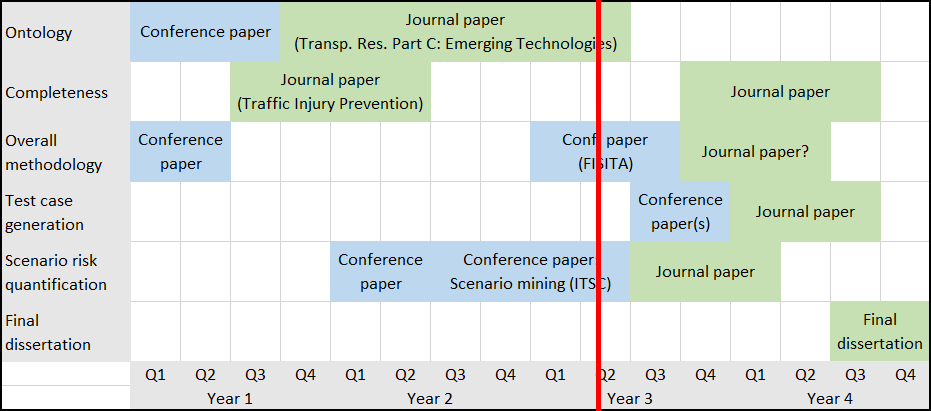
\includegraphics[width=\linewidth]{planning.png}
	\caption{Proposed planning at the time of this report. The red line indicated the time when writing this report.}
	\label{fig:planning}
\end{figure}

Note that, at some point, according to the planning in \cref{fig:planning}, I am working at four journal papers at the same time. I am not sure whether this is realistic. To make the planning less tight, I consider the following possibilities:
\begin{itemize}
	\item Skip the conference paper(s) for the ``test case generation'' and to go directly for a journal paper. 
	\item Skip the journal paper for ``completeness'', because I have already a journal paper on this subject.
\end{itemize}

On the short term, I plan to work on the following:
\begin{itemize}
	\item Submit the conference paper on scenario mining to ITSC.
	\item Continue the work on the scenario risk quantification and start writing the journal paper.
	\item Continue with a literature study for the test case generation and try out some ideas.
	\item Continue the internal discussion for a project with a car manufacture to apply the work of my PhD to assess an automated driving function.
\end{itemize}

\section{Questions}

\begin{itemize}
	\item For the ontology article, the status is ``waiting for decision'' since December 10, 2019. Could it be that the editor-in-chief simply forgot to decide? Could I send the editor-in-chief (Larry Head) an email to check the current status?
\end{itemize}


\printbibliography

\clearpage
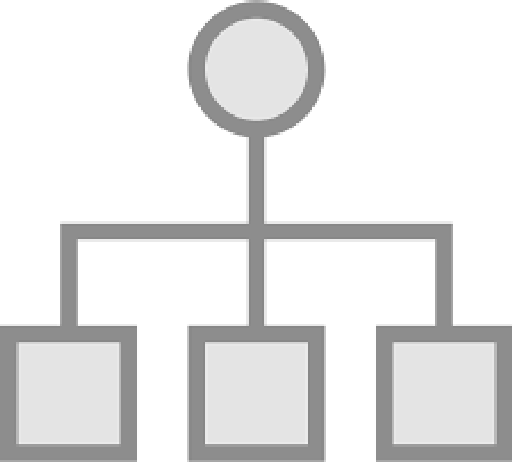
\includepdf[pages=-,pagecommand={},width=\paperwidth]{../../"20191010 Scenario Mining"/scenario_mining.pdf}

\end{document}